\subsection{The Intuition}
    
    \paragraph{Order Between Symmetric Threads}
        \begin{itemize}
            \item Symmetric executions can be obtained by swapping thread identities.
            \item Hence without loss of generality, we can assume a single total order of all threads which have equal code.
            \item In this sense, each set of equal threads will have a total order assigned to them. 
        \end{itemize}

    \paragraph{Order between Events - Writes and Reads}
        \begin{itemize}
            \item Whenever a read-write relation implies an order between two writes in a symmetric thread, swapping their thread identities will give us a symmetric execution with the order between writes reversed.
            \item Hence maintaining a symmetric order between writes of threads with equal code might be useful. 
            \item However, do we need a fixed order between all writes or just among writes which are equal in each thread? 
            \item Order between reads may not be necessary as they are not implied due to any other ordering-relation.  
        \end{itemize}

    \critic{red}{Whether order between reads is important is something I have a counter example to show that it isn't. But  I am not able to understand why it isn't important.}

    \paragraph{Miscellaneous Points}

        About ordering between writes through reads. 
        \begin{itemize}
            \item Each thread's read can read from it's own write program ordered before it.
            \item Each thread's read can read from an outer write which implies an ordering between the writes in it's own thread and the external one from which it reads from. 
        \end{itemize}

        \begin{figure}[H]
            \centering
            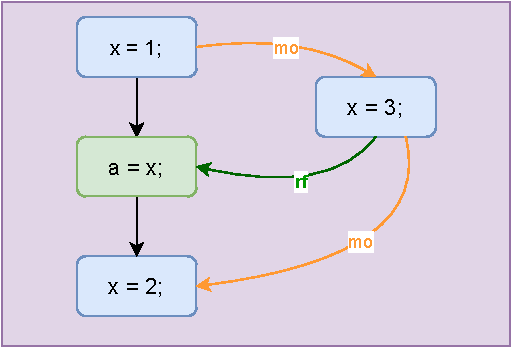
\includegraphics[scale=0.7]{WriteOrderImplied.pdf}
            \caption{Example showing that write orders(mo) implied due to the read-write(rf) relation.}
        \end{figure}




























   